\documentclass{article} % Document class definition

% Preamble starts here
\usepackage{amsmath}
\usepackage{graphicx}
\usepackage{needspace}
\setlength{\parskip}{1em} % Adds 1em space between paragraphs

\newenvironment{mpage}
  {\hspace{0.1in}
   \begin{minipage}{4.5in}
     \setlength{\parskip}{.5em}
     \vspace{0.1in}}    
  {\vspace{0.1in}
   \end{minipage}}


\title{Homework 4 Answers}
% \date{Due date: 10/26/2023 at 11:59 PM}
\author{}

\begin{document}
\maketitle

% Redefine the label for the top-level items
\renewcommand{\labelenumi}{Problem \arabic{enumi}}

% Redefine the label for the second-level items
\renewcommand{\labelenumii}{\alph{enumii})}


\begin{enumerate}

\item (1 point each) is Problem 1 in Discussion Questions in 4.26.  of
  *Problem Solving with Algorithms and Data Structures using Python*.
  Put the answer in a text file named \verb|hw3_last_first/p1.txt|.
  Convert the following values to binary using “divide by 2.” Show the
  stack of remainders.


  \begin{enumerate}
  \item
      % needspace ensurese there is at least 5 lines worth of space after
      % the 17
      \needspace{5\baselineskip} % Enough room for first few lines of answer.
      17

      \begin{mpage}
        ANSWER
        
        \begin{eqnarray*}
          17 / 2 &=& 8 r 1 \text{ push 1, stack: [1]} \\
          8 / 2  &=& 4 r 0 \text{ push 0, stack: [1, 0]} \\
          4 / 2  &=& 4 r 0 \text{ push 0, stack: [1, 0, 0]} \\
          2 / 2  &=& 2 r 0 \text{ push 0, stack: [1, 0, 0, 0]} \\
          1 / 2  &=& 0 r 1 \text{ push 1, stack: [1, 0, 0, 0, 1]} 
        \end{eqnarray*}

        Now pop the stack until empty to obtain the binary number: 10001.

        It is not required that the answer be presented exact as above.

        Any notion of the stack [1, 0, 0, 0, 1] is adequate.
        \vspace{.1in}

      \end{mpage}

    
    \item
        \needspace{5\baselineskip} % Enough room for first few lines of answer.
        45
      
        \begin{mpage}
          ANSWER

          \begin{eqnarray*}
            45 / 2 &=& 22 r 1 \text{ push 1, stack: [1]} \\
            22 / 2  &=& 11 r 0 \text{ push 0, stack: [1, 0]} \\
            11 / 2  &=& 5 r 1 \text{ push 1, stack: [1, 0, 1]} \\
            5 / 2  &=& 2 r 1 \text{ push 1, stack: [1, 0, 1, 1]} \\
            2 / 2  &=& 1 r 0 \text{ push 0, stack: [1, 0, 1, 1, 0]} \\
            1 / 2  &=& 1 r 1 \text{ push 1, stack: [1, 0, 1, 1, 0, 1]} 
          \end{eqnarray*}

          Now pop the stack until empty to obtain the binary number: 101101

          \vspace{.1in}
        \end{mpage}

    \item
      \needspace{5\baselineskip} % Enough room for first few lines of answer.
        96
      
        \begin{mpage}
          ANSWER
          
          \begin{eqnarray*}
            96 / 2 &=& 48 r 0 \text{ push 0, stack: [0]} \\
            48 / 2 &=& 24 r 0 \text{ push 0, stack: [0, 0]} \\
            24 / 2 &=& 12 r 0 \text{ push 0, stack: [0, 0, 0]} \\
            12 / 2 &=& 6 r 0  \text{ push 0, stack: [0, 0, 0, 0]} \\
            6 / 2 &=& 3 r 0   \text{ push 0, stack: [0, 0, 0, 0, 0]} \\
            3 / 2 &=& 1 r 1   \text{ push 1, stack: [0, 0, 0, 0, 0, 1]} \\
            1 / 2 &=& 0 r 1   \text{ push 1, stack: [0, 0, 0, 0, 0, 1, 1]}
          \end{eqnarray*}

          Now pop the stack util empty to obtain the binary number 1100000.

          \vspace{.1in}
        \end{mpage}

  \end{enumerate}

\item (2 points)

  \begin{enumerate}
    \needspace{5\baselineskip} % Enough room for first few lines of answer.
    \item Create a \verb|LinkedList| class.  It must pass the
      \verb|hw3/p2/test_linked_list.py|.  The class MUST not use any
      Python built-in or standard library collection class, i.e., do
      not wrap a list or deque.
  
      \begin{mpage}
        ANSWER

        I included an implementation of \verb|linked_list.py| in the
        repository.  The answer provided by the student must pass
        \verb|test_linked_list.py|.
        \vspace{.1in}
      \end{mpage}

  \item   Copy the Stack implementation found in the
  repository

  \begin{verbatim}
    https://git.cs.olemiss.edu/harrison/csci-356
  \end{verbatim}

  in \verb|lecture13and14/stack.py| into your homework directory
  \verb|hw3_last_first/p2|, rename the class \verb|LinkedListStack|
  and modify it so that it is implemented using your \verb|LinkedList|. It
  must pass the unit tests in the repository in the directory
  \verb|hw3/test_linked_stack.py|.  It MUST use your LinkedList.  the
  new Stack class MUST NOT use any Python built-in or standard library
  collection class, i.e., the \verb|LinkedListStack| class MUST not wrap a
  \verb|list| or \verb|deque|.

      \begin{mpage}
        ANSWER

        I included an implementation of \verb|linked_list_stack.py| in
        the repository in \verb|hw3/|.  The answer provided by the
        student must pass \verb|test_linked_list.py|.
        \vspace{.1in}
      \end{mpage}

      
  \end{enumerate} 

\item (1 point each)
  Problem 3 in Discussion Questions in 4.26 of *Problem Solving with
  Algorithms and Data Structures using Python*. 

  Convert the infix expressions to postfix (use full parentheses).

  \begin{enumerate}
  \item \label{infix2post}
    \needspace{5\baselineskip}
    \verb|(A+B)*(C+D)*(E+F)|

    \begin{mpage}
      ANSWER

      The book suggests the following procedure:

      \begin{quotation}
        
        1. Create an empty stack called opstack for keeping
        operators. Create an empty list for output.

        2. Convert the input infix string to a list by using the string
        method split.

        3. Scan the token list from left to right.

        4. If the token is an operand, append it to the end of the output list.

        5. If the token is a left parenthesis, push it on the opstack.

        6. If the token is a right parenthesis, pop the opstack until the
        corresponding left parenthesis is removed. Append each
        operator to the end of the output list.

        7. If the token is an operator, *, /, +, or -, push it on the
        opstack. However, first remove any operators already on the
        opstack that have higher or equal precedence and append them
        to the output list.

        When the input expression has been completely processed, check
        the opstack. Any operators still on the stack can be removed
        and appended to the end of the output list.
      \end{quotation}
    \end{mpage}

    \begin{mpage}
      The input is \verb|(A+B)*(C+D)*(E+F)|, which is processed as follows

        \begin{verbatim}
          (A+B)*(C+D)*(E+F)  opstack = [], output=""
          A+B)*(C+D)*(E+F)   opstack = ['('], output=""
          +B)*(C+D)*(E+F)    opstack = ['('], output="A"
          B)*(C+D)*(E+F)     opstack = ['(', '+'], output="A"
          )*(C+D)*(E+F)      opstack = ['(', '+'], output="AB"
          *(C+D)*(E+F)       opstack = [], output="AB+"
          (C+D)*(E+F)        opstack = ['*'], output="AB+"
          C+D)*(E+F)         opstack = ['*', '('], output="AB+"
          +D)*(E+F)          opstack = ['*', '('], output="AB+C"
          
          D)*(E+F)           opstack = ['*', '(', '+'], output="AB+C"
          )*(E+F)            opstack = ['*', '(', '+'], output="AB+CD"
          *(E+F)             opstack = ['*'], output="AB+CD+"
          (E+F)              opstack = ['*'], output="AB+CD+*"
          E+F)               opstack = ['*', '('], output="AB+CD+*"
          +F)                opstack = ['*', '('], output="AB+CD+*E"
          F)                 opstack = ['*', '(', '+'], output="AB+CD+*E"
          )                  opstack = ['*', '(', '+'], output="AB+CD+*EF"
                             opstack = [], output="AB+CD+*EF+*"
        \end{verbatim}
         
        So the postfix generated by the algorithm presented in the book is
        given by
        
\begin{verbatim}
  AB+CD+*EF+*
\end{verbatim}

      \vspace{.1in}
    \end{mpage}

  \item
    \needspace{5\baselineskip} % Enough room for first few lines of answer.
    \verb|A+((B+C)*(D+E))|
    
    \begin{mpage}
      ANSWER

      Using the analogous procedure given for the conversion
      for Problem~\ref{infix2post}, we generate the following postfix:

        \begin{verbatim}
          ABC+DE+*+
        \end{verbatim}

      \vspace{.1in}
    \end{mpage}

      
  \item
    \needspace{5\baselineskip} 
    \verb|A*B*C*D+E+F|

    \begin{mpage}
      ANSWER

      The procedure in the book would provide the following result:
      
        \begin{verbatim}
          AB*C*D*E+F+|
        \end{verbatim}

      However, the following is an equivalent postfix notation for the given
      mathematical expression:

        \begin{verbatim}
          ABCD***EF++
        \end{verbatim}

      All variants that produce the same result should be accepted.

    \end{mpage}

  \end{enumerate}


  % Problem 4
  \item (2 points) Use the `Queue` found in the source code
repository in `hw3/p4/queue.py`, which is based on the code in the
book in Listing 1 of Section 4.12


    \begin{enumerate}
  
    \item Create file \verb|perftest_list_queue_a.py| in
      \verb|hw3_last_first/p4| whose \verb|main| function enqueues $n$
      random integers into $m$ Queue objects according to the following
      pseudocode:

\begin{verbatim}
  create m empty `Queue` objects and put them in a list named queues.
  for n in some range:
      start timer
          for x in queues:
              enqueue the nth random integer into queue x
      stop timer
      divide the elapsed time by m to get an average
      append the average time for an execution of enqueue to a list of times.
\end{verbatim}

      Using \verb|matplotlib| have your code plot the average
      execution time for a call to \verb|enqueue()| as a function of
      $n$.  Vary $n$ at least to 10,000.  You may skip $n$ by
      increments of 10, but if you do then adjust the x-axis
      accordingly.

      \begin{mpage}
        ANSWER

        I committed my version of \verb|perftest_list_queue_a.py| in
        the \verb|csci-356| repository in the directory \verb|hw3/p4/|.
      
        The student should deliver a plot that looks linear as in 
        Figure~\ref{fig:hw3_p4_enq_vs_n}.

      \end{mpage}

      \begin{figure}[ht]
        \centering
        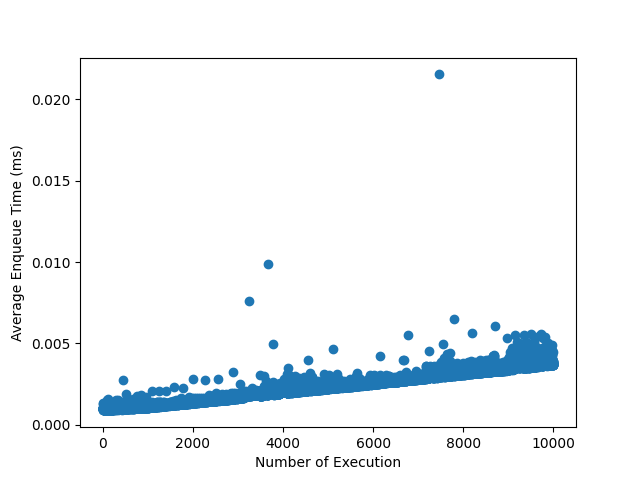
\includegraphics[width=\linewidth]{p4/enq_run_time_vs_n.png}
        \caption{Problem 4: The average run time per call to enqueue
          for the Queue class.}
        \label{fig:hw3_p4_enq_vs_n}
      \end{figure}

    \item Analyze the performance of the \verb|enqueue()| method using
      big-O notation.  Put your analysis in a file named
      \verb|hw3_last_first/p4/b.txt|.

      \begin{mpage}
        ANSWER

        The Queue uses a Python list as the underlying data structure.
        The analysis is simple.

\begin{verbatim}
  
          def enqueue(self, item) -> None:
              self.items.insert(0,item)     // O(n)
\end{verbatim}

        Since the \verb|insert| is $O(n)$, \verb|enqueue| is $O(n)$.
      \end{mpage}

    \item In a file \verb|perftest_list_queue_c.py| Create a variant
      of the code created for (a) that starts by creating $m$ Queues
      of the largest length (e.g., $n=10000$) and then dequeues one
      item from each list while recording the average time for a
      dequeue.  Using \verb|matplotlib| plot the average execution
      time for a call to \verb|dequeue()| as a function of $n$.  If it
      runs too slowly you can start with $n=1000$.  You may skip $n$
      by increments of 10, but if you do then adjust the x-axis
      accordingly.

      \begin{mpage}
        ANSWER

        I committed my version of \verb|perftest_list_queue_c.py| in
        the \verb|csci-356| repository in the directory \verb|hw3/p4/|.
      
        The student should deliver a plot that looks like performance
        is $O(1)$ as in Figure~\ref{fig:hw3_p4_enq_vs_n}.  In
        Figure~\ref{fig:hw3_p4_enq_vs_n}, there are a few spikes.
        I have run this with different seeds, and the spikes appear in the
        same place and they persist even if garbage collection is turned
        off.  This could be due to shrinking the list's underlying array
        as the list shrinks.  This would be consistent with list having
        amortized $O(1)$ time complexity.

      \end{mpage}


      \begin{figure}[ht]
        \centering
        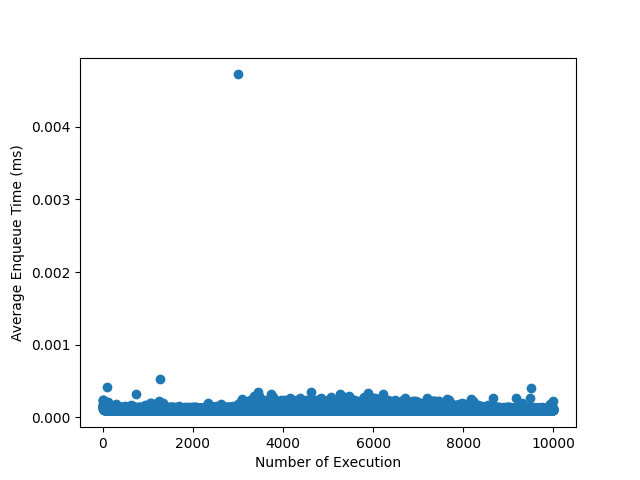
\includegraphics[width=\linewidth]{p4/deq_run_time_vs_n.png}
        \caption{Problem 4: The average run time per call to dequeue
          for the Queue class.}
        \label{fig:hw3_p4_deq_vs_n}
      \end{figure}

    \item Analyze the performance of the \verb|dequeue()| method using
      big-O notation and put your analysis in a file named
      \verb|hw3_last_first/p4/d.txt|.

      \begin{mpage}
        ANSWER

        The Queue uses a Python list as the underlying data structure.
        The analysis is simple.

        \begin{verbatim}
          def dequeue(self) -> object:
            return self.items.pop()      # O(1)
        \end{verbatim}

        Since the \verb|pop| is $O(1)$, \verb|dequeue| is $O(1)$.
        However, as indicated in the plot and with our prior knowledge
        of the Python list being a dynamic vector (a.k.a., dynamic
        array), we should see some spikes as the Queue shrinks which
        would be consistent with the Python list reallocating to a
        smaller array and copying the elements from the old array to
        the new one.

        If the student specifies $O(1)$ this is good enough, but kudos
        to those that state amortized $O(1)$.
        
      \end{mpage}
    \end{enumerate}


  \item (1 point) is Problem 5 in Discussion Questions in 4.26.  of
    *Problem Solving with Algorithms and Data Structures using
    Python*.  I copy the problem below:

    \begin{quotation}
    Evaluate the following postfix expressions. Show the stack as each
    operand and operator is processed.
    \end{quotation}

    \begin{enumerate}
    \item
      \needspace{5\baselineskip} % Enough room for first few lines of answer.
      \verb|2 3 * 4 +|
      
      \begin{mpage}
        ANSWER
        
        \vspace{0.1in} We push every encountered
        number in the input stream into the stack until we encounter
        a mathematical operator at such point, we pop the last two numbers,
        perform the mathematical operation and push the result onto the
        stack.  When there are no more characters in the input stream,
        the stack should have a depth of 1 and this element is the result.

\begin{verbatim}
         2 3 * 4 +    stack=[]
           3 * 4 +    stack=[2]
             * 4 +    stack=[2, 3]
               4 +    stack=[6]
                 +    stack=[6, 4]
                      stack=[10]
\end{verbatim}
    
        The result of evaluating the expression is 10.
      \end{mpage}

    \item
      \needspace{5\baselineskip} % Enough room for first few lines of answer.
      \verb|1 2 + 3 + 4 + 5 +|

      \begin{mpage}
        ANSWER

\begin{verbatim}
        1 2 + 3 + 4 + 5 +    stack=[]
          2 + 3 + 4 + 5 +    stack=[1]
            + 3 + 4 + 5 +    stack=[1, 2]
              3 + 4 + 5 +    stack=[3]
                + 4 + 5 +    stack=[3, 3]
                  4 + 5 +    stack=[6]
                    + 5 +    stack=[6, 4]
                      5 +    stack=[10]
                        +    stack=[10, 5]
                             stack=[15]
\end{verbatim}

        \vspace{.1in}
      \end{mpage}

    \item
      \needspace{5\baselineskip} % Enough room for first few lines of answer.
      \verb|1 2 3 4 5 * + * +|

      \hspace{.1in}
      \begin{mpage}
        \vspace{.1in}
        ANSWER

\begin{verbatim}
        1 2 3 4 5 * + * +    stack=[]
          2 3 4 5 * + * +    stack=[1]
            3 4 5 * + * +    stack=[1, 2]
              4 5 * + * +    stack=[1, 2, 3]
                5 * + * +    stack=[1, 2, 3, 4]
                  * + * +    stack=[1, 2, 3, 4, 5]
                    + * +    stack=[1, 2, 3, 20]
                      * +    stack=[1, 2, 23]
                        +    stack=[1, 46]
                             stack=[47]
\end{verbatim}

        The result of evaluating the expression is 47.

      \end{mpage}

    \end{enumerate}


  \item Repeat problem 4, but implement a Queue using a Python deque
    (a.k.a., doubly-ended queue). Generate the plots and analyze the
    enqueue and dequeue methods using big-O notation in the same
    manner. In the plots for (a) and (c) include the plot for the same
    scenario but using the list implementation of the Queue. This way
    we can visually compare the performance of the list and deque
    implementations.

    \begin{mpage}
      ANSWER

      The Queue uses a Python deque as the underlying data structure.
      The analysis enqueue is simple.

\begin{verbatim}
         def enqueue(self) -> object:
             return self.items.append()      # O(1)
\end{verbatim}

      Thus the \verb|enqueue| call is $O(1)$.

      Your enqueue can append to the front or the rear as long
      as the deqeue pops from the opposite end.

      Similar argument applies for \verb|dequeue|.
      
\begin{verbatim}
         def dequeue(self) -> object:
             return self.items.popleft()      # O(1)
\end{verbatim}

      Thus the \verb|deque| call is also $O(1)$.

      This time BOTH plots should show $O(1)$ behavior similar
      to what appear in Figure~\ref{fig:hw3_p6_enq_vs_n} and
      Figure~\ref{fig:hw3_p6_deq_vs_n}.

      However, as indicated in the plot and with our prior knowledge
      of the Python list being a dynamic vector (a.k.a., dynamic
      array), we should see some spikes as the Queue shrinks which
      would be consistent with the Python list reallocating to a
      smaller array and copying the elements from the old array to
      the new one.

      If the student specifies $O(1)$ this is good enough, but kudos
      to those that state amortized $O(1)$.

    \end{mpage}

    \begin{figure}[ht]
      \centering
      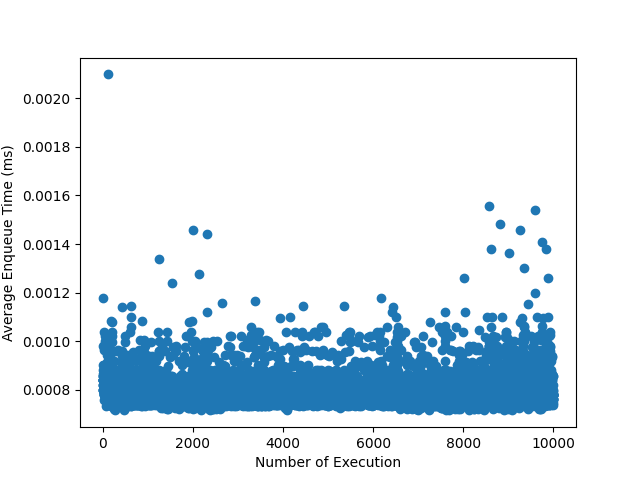
\includegraphics[width=\linewidth]{p6/deque_enq_run_time_vs_n.png}
      \caption{Problem 6: The average run time per call to enqueue
        for the deque-based Queue class.}
      \label{fig:hw3_p6_enq_vs_n}
    \end{figure}

    \begin{figure}[ht]
      \centering
      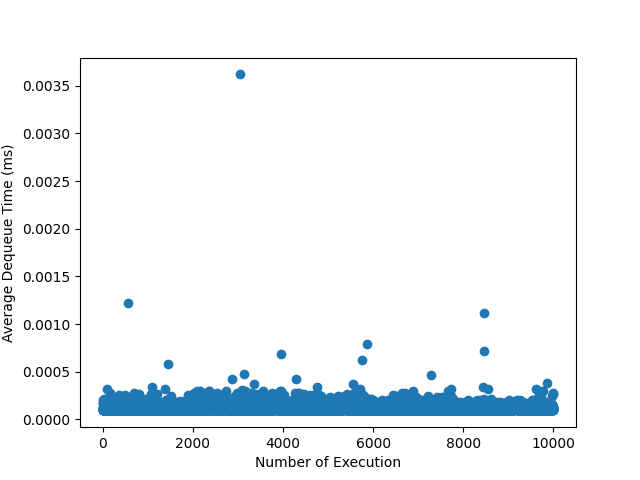
\includegraphics[width=\linewidth]{p6/deque_deq_run_time_vs_n.png}
      \caption{Problem 6: The average run time per call to dequeue
        for the deque-based Queue class.}
      \label{fig:hw3_p6_deq_vs_n}
    \end{figure}


\item (1 point) is Problem 11 in Programming Exercises in 4.27.
of *Problem Solving with Algorithms and Data Structures using Python*.
It must pass the unit tests for \verb|p7/test_html_balance.py|.

  \begin{quotation}
Another example of the parentheses matching problem comes from
hypertext markup language (HTML). In HTML, tags exist in both opening
and closing forms and must be balanced to properly describe a web
document. This very simple HTML document:
  \end{quotation}

  \begin{verbatim}
    <html>
       <head>
          <title>
             Example
          </title>
       </head>
    
       <body>
          <h1>Hello, world</h1>
       </body>
     </html>
  \end{verbatim}

  is intended only to show the matching and nesting structure for tags
  in the language. Write a program that can check an HTML document for
  proper opening and closing tags.

  \begin{mpage}
    ANSWER

    I committed my answer to this question in
    \verb|hw3/p7/test_html_balance.py|.

    The student's answer should pass the tests in \verb|test_html_balance.py|.
    
  \end{mpage}


\end{enumerate}


\end{document}
